
%--------------------------------------------------------------------
\section{Introduction}
%--------------------------------------------------------------------

\begin{frame}
    \frametitle{Introduction}
    \framesubtitle{Overview of Dissertation}

    This dissertation explores the possibilites and develops 
    algorithms for 
    \begin{itemize}
        \item modeling human behaviors; 
        \item detecting anomalies 
    \end{itemize}
    \alert{without} requiring large databases of training data. 
  
\end{frame}

%--------------------------------------------------------------------

\begin{frame}
    \frametitle{Introduction}
    \framesubtitle{Background and Motivation}

    \begin{itemize}
        \item Video surveillance is ubiquitous in our lives and 
            more important for preventing and responding 
            criminal activities.
        \item Resulting proliferation of surveillance cameras becomes 
            a problem to monitor all channels.
        \item Human monitoring is therefore expensive and ineffective. 
    \end{itemize}

    \begin{figure}
        \centering
        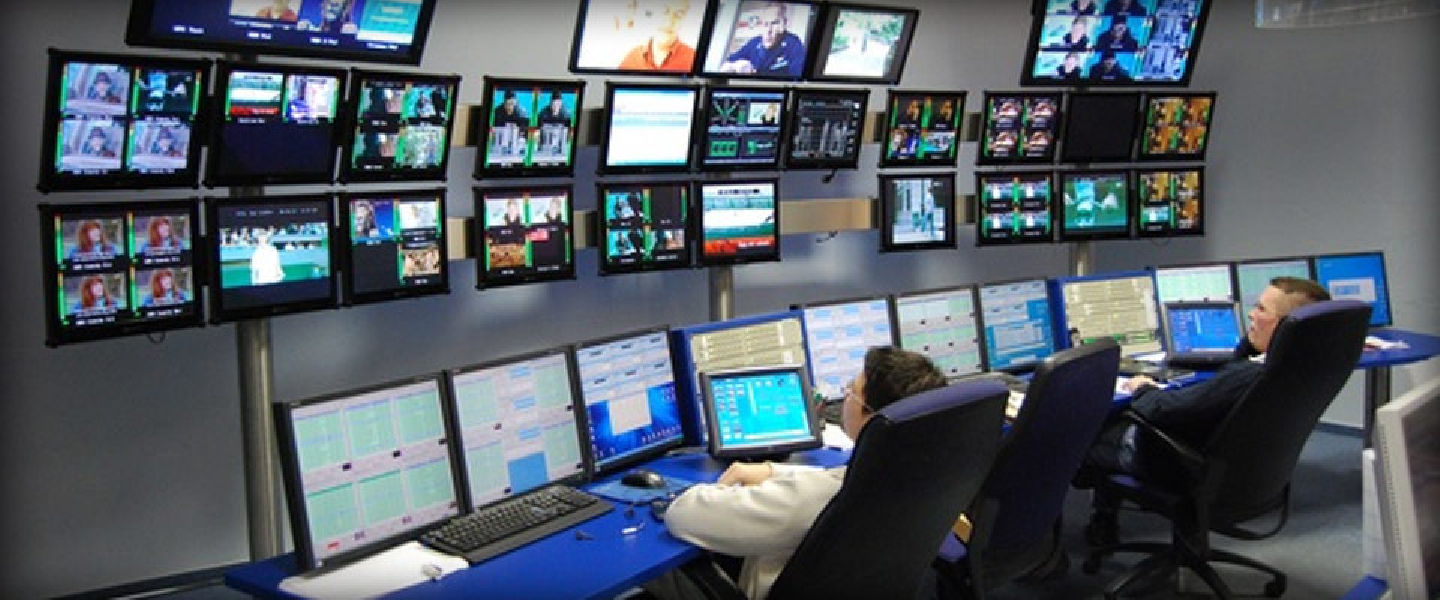
\includegraphics[width=2.5in]{figures/monitoring}
        \caption{CCTV monitoring room. Reprinted from the Twenty First 
            Security Web site.}
    \end{figure}
  
\end{frame}

%--------------------------------------------------------------------

\begin{frame}
    \frametitle{Introduction}
    \framesubtitle{Problems in Existing Work}

    \begin{itemize}
        \item Existing work learns behaviors in batch mode and creates 
            separate models, which remain static once trained, for each 
            distinct class of behavior.
        \item The number of ``normal'' behaviors needs to be known 
            beforehand because we cannot learn a model for ``abnormal'' 
            behavior that is rare and diverse.
        \item A behavior considered {\em normal} in one context might be 
            considered {\em abnormal} in another context depending on the type 
            of behavior and where and when it is observed.
    \end{itemize}

\end{frame}

%--------------------------------------------------------------------

\begin{frame}
    \frametitle{Introduction}
    \framesubtitle{Challenges}

    \begin{enumerate}
        \item It is impractical to store all data.
            \begin{itemize}
                \item[-] Need an efficient method that learns scene-speific 
                    statistical models of human behavior \alert{without} 
                    requiring storage of databases of training data.
             \end{itemize}
        \item Real human behavior is sometimes ambiguous. 
            \begin{itemize}
                \item[-] Need to keep humans in the loop to interpret it.
            \end{itemize}
        \item Unusual behavior is rare and diverse. 
            \begin{itemize}
                \item[-] Impractical to acquire sufficient data 
                    for a good model for it; 
                \item[-] Need to detect deviations from typical behavior.
            \end{itemize}
    \end{enumerate}
  
\end{frame}

%--------------------------------------------------------------------

\begin{frame}
    \frametitle{Introduction}
    \framesubtitle{Challenges (cont.)}

    We propose an efficient method for 
    automatic identification of suspicious behavior that 
    \alert{incrementally} learns scene-specific statistical models 
    of human behavior \alert{without} requiring storage of 
    large databases of training data.

    \bigskip

    Our method is based on hidden Markov models (HMMs) with 
    \alert{sufficient statistics} and an optimal threshold 
    on the likelihood of an event according to the human behavior model.

\end{frame}
    
%--------------------------------------------------------------------

\ifnum\short=0

\begin{frame}
    \frametitle{Introduction}
    \framesubtitle{Overview of Methodology}
   
    \begin{enumerate}
        \item We begin by building an initial set of models explaining 
            the behaviors occurring in a small bootstrap data set.
        \item We partition the bootstrap set into clusters then assign 
            new observation sequences to cluster based on statistical 
            tests of HMM log likelihood scores.
        \item After bootstrapping, each new sequence is used to incrementally 
            update the sufficient statistics of the HMM it is assigned to. 
    \end{enumerate}

    \medskip

    Our method solves the problem of inducing 
    scene-specific statistical models useful for bringing suspicious 
    behavior to the attention of human security personnel.

\end{frame}

\fi

%--------------------------------------------------------------------

\begin{frame}
    \frametitle{Introduction}
    \framesubtitle{Contributions}

    The contributions of this dissertation are as follows.
    \begin{enumerate}
        \item Propose an intelligent video surveillance system that 
            is practical and fairly close to the ideal surveillance 
            system, which should monitor and automatically raise 
            alarms to security personnel; 
        \item Develop an algorithm for extracting and tracking 
            multiple moving foreground blobs using an appearance model; 
        \item Propose a shadow detection method that uses a simple 
            maximum likelihood classification approach based on color 
            information; 
        \item Propose a new method for clustering human behaviors 
            that is suitable for bootstrapping an 
            anomaly detection module for intelligent video surveillance 
            systems; 
    \end{enumerate}

\end{frame}

%--------------------------------------------------------------------

\begin{frame}
    \frametitle{Introduction}
    \framesubtitle{Contributions (cont.)}

    \begin{enumerate}
        \setcounter{enumi}{4}
        \item Propose and develop a new and effective algorithm 
            for semi-supervised learning of common human behaviors 
            and detect anomalies in video sequences; 
        \item Introduce a new and more accurate algorithm for 
            incrementally profiling human behaviors
            in video sequences without requiring storage of large databases 
            of training data; 
        \item Provide the source code and datasets online for researchers 
            interested in evaluating or
            extending our work.
    \end{enumerate}

\end{frame}

%--------------------------------------------------------------------

\begin{frame}
    \frametitle{Introduction}
    \framesubtitle{List of Publications}

    Published Works
    \begin{itemize}
        \item Clustering Human Behaviors with Dynamic Time Warping and 
            Hidden Markov Models for a Video Surveillance System 
            (ECTI-CON 2010)
        \item Automatic Suspicious Behavior Detection from a Small 
            Bootstrap Set (VISAPP 2012)
        \item Incremental Behavior Modeling and Suspicious Activity 
            Detection (PR 2013)
        \item Extracting the Object from the Shadows: Maximum Likelihood 
            Object/Shadow Discrimination (ECTI-CON 2013)
    \end{itemize}
    
    \medskip
    
    We plan to submit a paper ``Incorporating Geometric and Shadow 
    Region Shape Information for Shadow Detection'' to CVPR 2013.

\end{frame}

